%%
%% Based on "Как запускается функция main() в Linux"
%% http://www.linuxlib.ru/prog/mainlin.htm

\begin{frame}
	\frametitle{ELF}
	\begin{columns}
		\column{0.5\textwidth}
			\begin{block}{Executable and Linkable Format}
				Файлы могут включать:
				\begin{itemize}
					\item Таблицу Program Header,  описывающую ноль или более сегментов
					\item Таблицу Section Header,  описывающую ноль или более секций
					\item Данные,  упомянутые в записях названных таблиц
				\end{itemize}
			\end{block}
		\column{0.5\textwidth}
			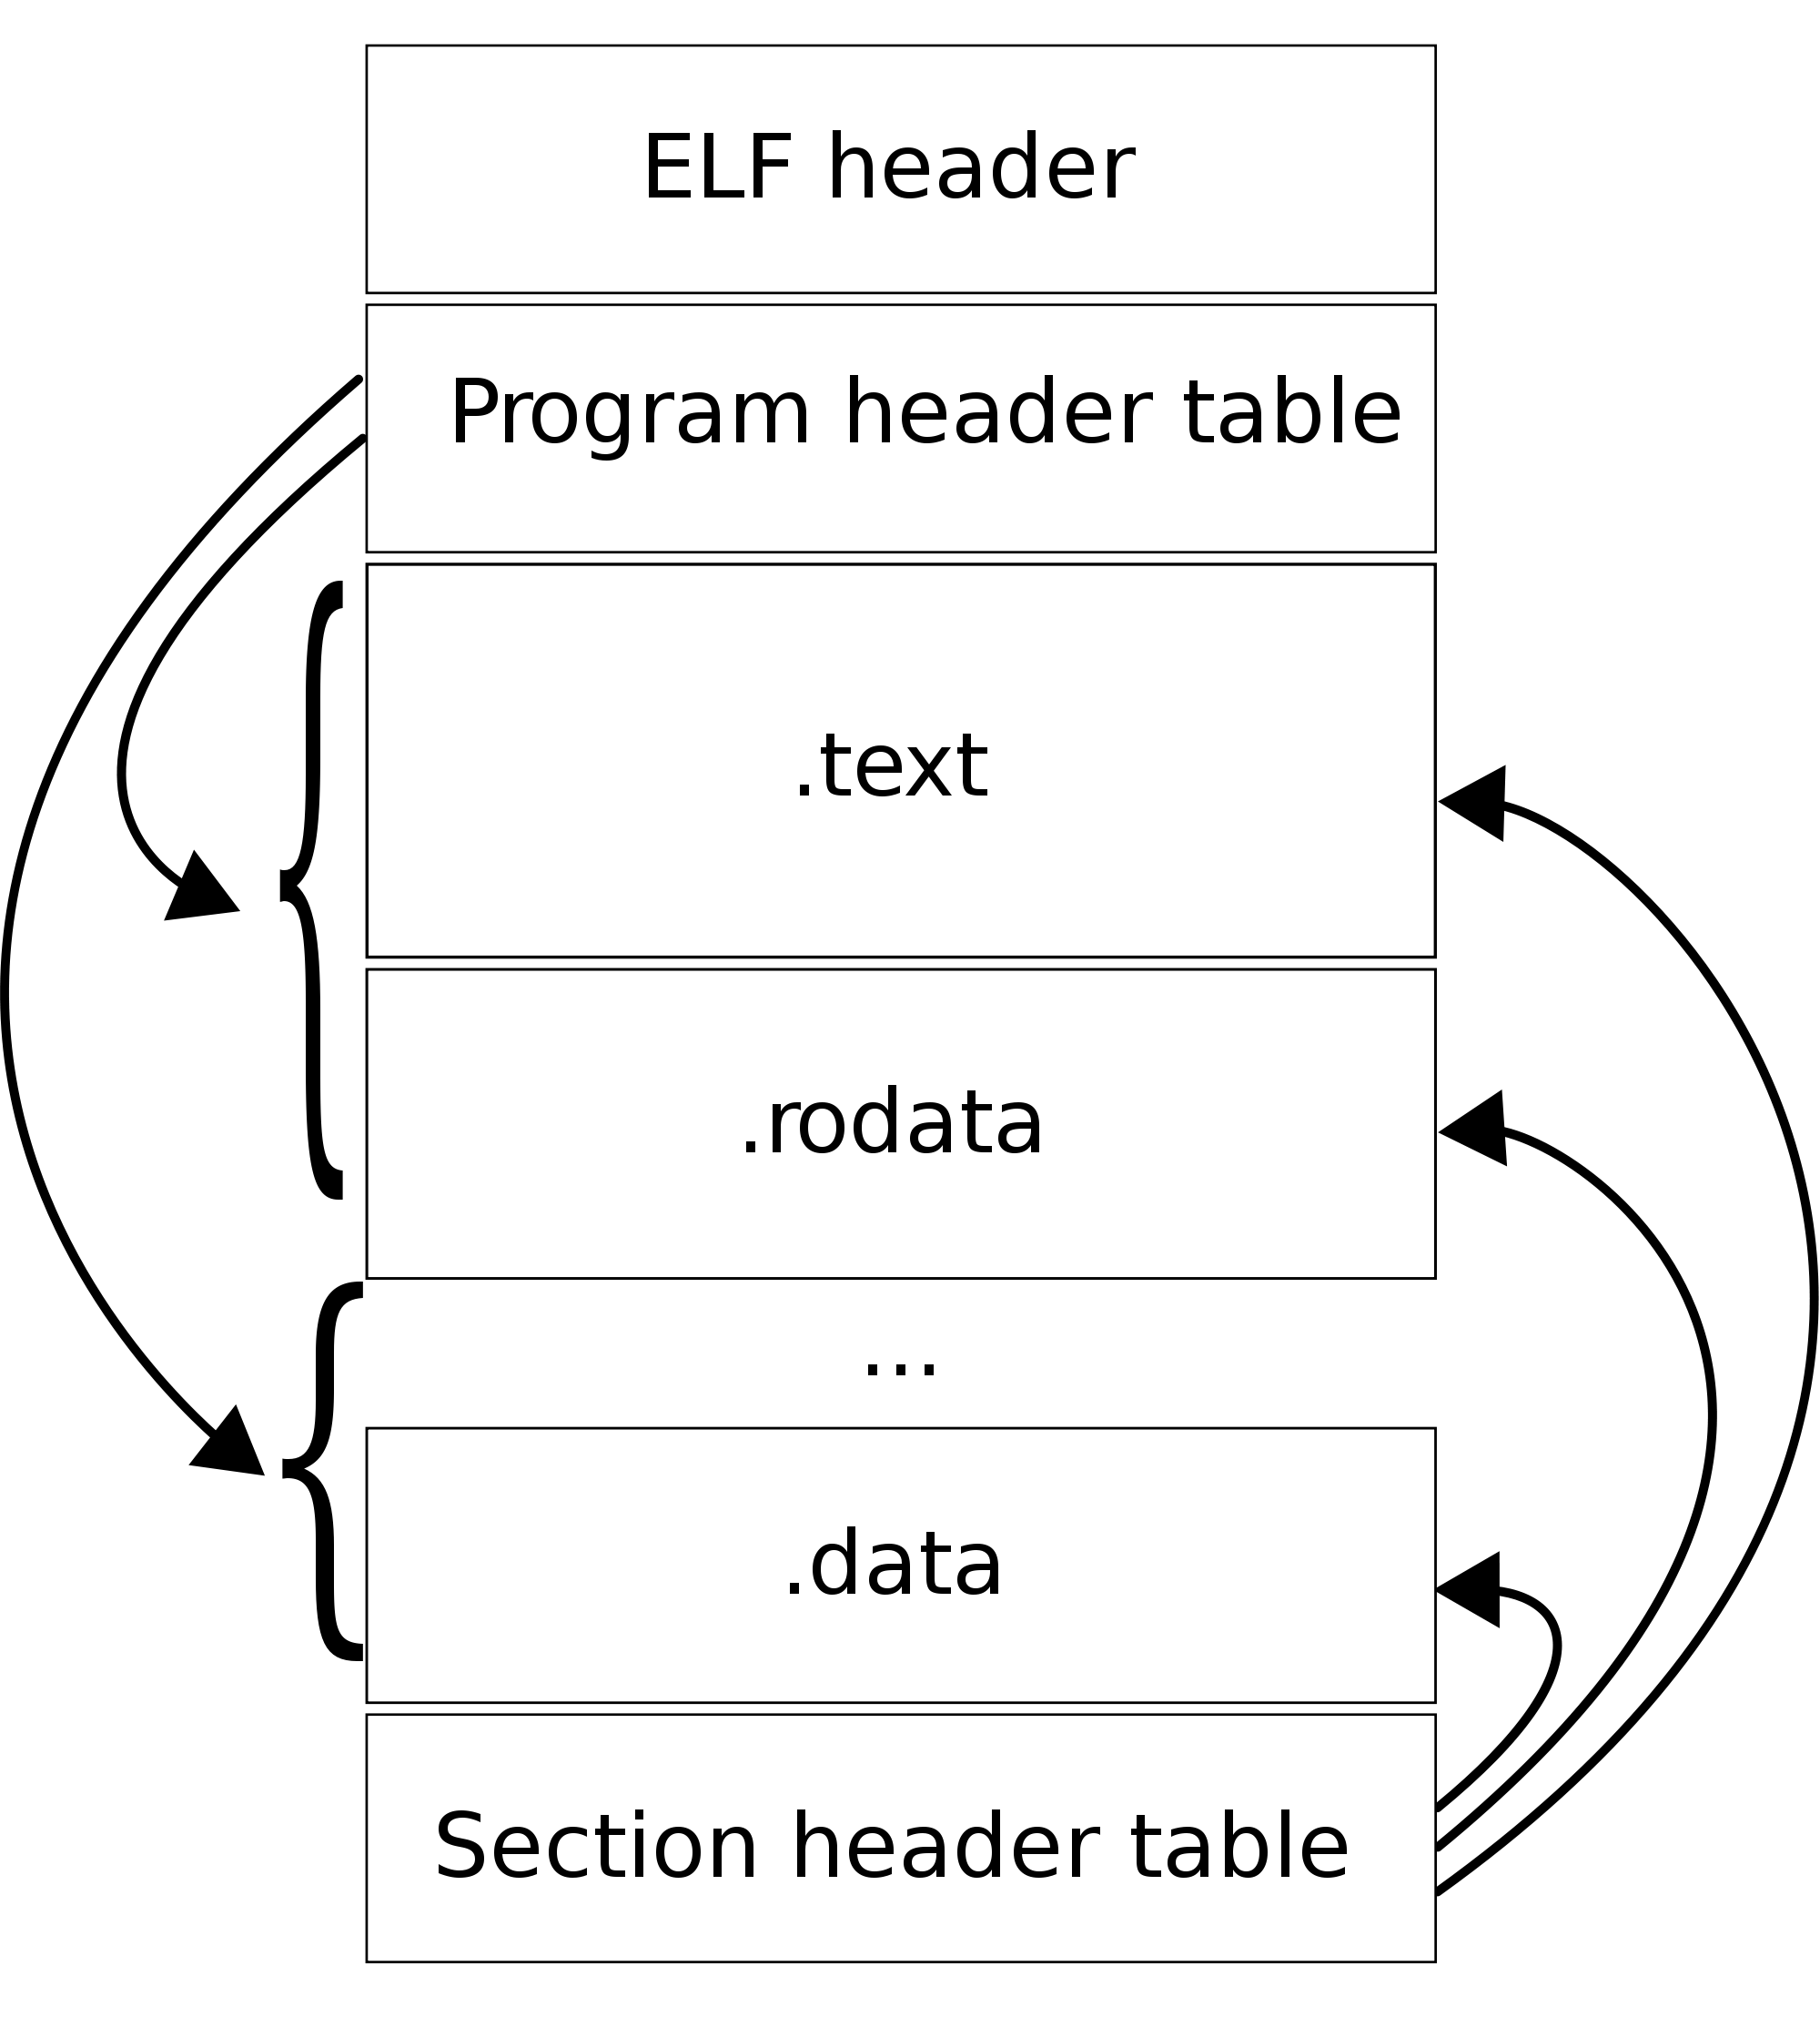
\includegraphics[height=0.8\textheight]{../../slides/elf-analysis/Elf-layout.png}
	\end{columns}
\end{frame}

\begin{frame}
	\frametitle{Запуск main()}

	\begin{block}{Пример}
		Для анализа понадобится пример из занятия по введению в gcc (последовательность линковки библиотек).
	\end{block}

	Пример доступен по адресу \url{https://github.com/d4s/linux\_courses/tree/master/epam/examples/make/linking}
	
\end{frame}

